\documentclass[11pt,a4paper]{article}
\usepackage[utf8]{inputenc}
\usepackage{amsmath}
\usepackage{amsfonts}
\usepackage{amssymb}
\usepackage{graphicx}
\usepackage{tikz}
\usetikzlibrary{fit,positioning}

\usepackage[left=1in,right=1in,top=1in,bottom=1in]{geometry}
\begin{document}

	\begin{figure}
	\begin{center}
	\begin{tabular}{|c|c|c|c|c|}
		\hline
		 & K-Means & GMM & DPGMM & Labeled \\
		 \hline
		 LDA & 0.9006 & 0.8486 & 0.8562 & 2000 \\
		 \hline
		 Bigram & 0.8135 & 0.7516 & 0.7536 & 200 \\
		 \hline
		 PCA & 0.9451 & 0.8 & 0.7969 & 500 \\
		 \hline
	\end{tabular}
	\caption{10 x 25}
	\end{center}
	\end{figure}





	\begin{figure}
	\begin{center}
	\begin{tabular}{|c|c|c|c|c|}
		\hline
		 & K-Means & GMM & DPGMM & Labeled \\
		 \hline
		 LDA & 0.8867 & 0.8790 & 0.8402 & 2200 \\
		 \hline
		 Bigram & 0.7356 & 0.7247 & 0.6438 & 200 \\
		 \hline
		 PCA & 0.927 & 0.8632 & 0.8746 & 600 \\
		 \hline
	\end{tabular}
	\caption{10 x 50}
	\end{center}
	\end{figure}
	
	
	
	\begin{figure}
	\begin{center}
	\begin{tabular}{|c|c|c|c|c|}
		\hline
		 & K-Means & GMM & DPGMM & Labeled \\
		 \hline
		 LDA & 0.8827 & 0.8967 & 0.8450 & 2000 \\
		 \hline
		 Bigram & 0.8 & 0.7400 & 0.7483 & 200 \\
		 \hline
		 PCA & 0.8932 & 0.8425 & 0.8522 & 600 \\
		 \hline
	\end{tabular}
	\caption{10 x 100}
	\end{center}
	\end{figure}
	
	
	
	\begin{figure}
	\begin{center}
	\begin{tabular}{|c|c|c|c|c|}
		\hline
		 & K-Means & GMM & DPGMM & Labeled \\
		 \hline
		 LDA & 0.9088 & 0.8840 & 0.8899 & 1500 \\
		 \hline
		 PCA & 0.9829 & & 0.8190 & 400 \\
		 \hline
	\end{tabular}
	\caption{25 x 25}
	\end{center}
	\end{figure}
	
	
	
	\begin{figure}
	\begin{center}
	\begin{tabular}{|c|c|c|c|c|}
		\hline
		 & K-Means & GMM & DPGMM & Labeled \\
		 \hline
		 LDA & 0.9081 & 0.875 & 0.8686 & 1700 \\
		 \hline
		 PCA & 0.9065 & & 0.8469 & 600 \\
		 \hline
	\end{tabular}
	\caption{25 x 50}
	\end{center}
	\end{figure}
	
	
	
	\begin{figure}
	\begin{center}
	\begin{tabular}{|c|c|c|c|c|}
		\hline
		 & K-Means & GMM & DPGMM & Labeled \\
		 \hline
		 LDA & 0.9210 & 0.8492 & 0.8721 & 2000 \\
		 \hline
	\end{tabular}
	\caption{25 x 100}
	\end{center}
	\end{figure}
	
	
	
	\begin{figure}
	\begin{center}
	\begin{tabular}{|c|c|c|c|c|}
		\hline
		 & K-Means & GMM & DPGMM & Labeled \\
		 \hline
		 LDA & 0.8802 & 0.8974 & 0.8685 & 1200 \\
		 \hline
		 PCA & 0.8802 & & 0.8653 & 700 \\
		 \hline
	\end{tabular}
	\caption{50 x 25}
	\end{center}
	\end{figure}
	
	
	
	\begin{figure}
	\begin{center}
	\begin{tabular}{|c|c|c|c|c|}
		\hline
		 & K-Means & GMM & DPGMM & Labeled\\
		 \hline
		 LDA & 0.8726 & 0.8589 & 0.8288  & 1400 \\
		 \hline
		 PCA & 0.9229 & & & 600 \\
		 \hline
	\end{tabular}
	\caption{50 x 50}
	\end{center}
	\end{figure}
	
	
	
	\begin{figure}
	\begin{center}
	\begin{tabular}{|c|c|c|c|c|}
		\hline
		 & K-Means & GMM & DPGMM & Labeled\\
		 \hline
		 LDA & 0.8851 & 0.8683 & 0.8500 & 1400  \\
		 \hline
		 PCA & 0.9122 & & & 700 \\
		 \hline
	\end{tabular}
	\caption{50 x 100}
	\end{center}
	\end{figure}
	
	
	\begin{figure}
		\begin{center}
			\includegraphics[scale=1.0]{lda_bigram_compare}
		\end{center}
	\end{figure}

	\begin{figure}
		\begin{center}
			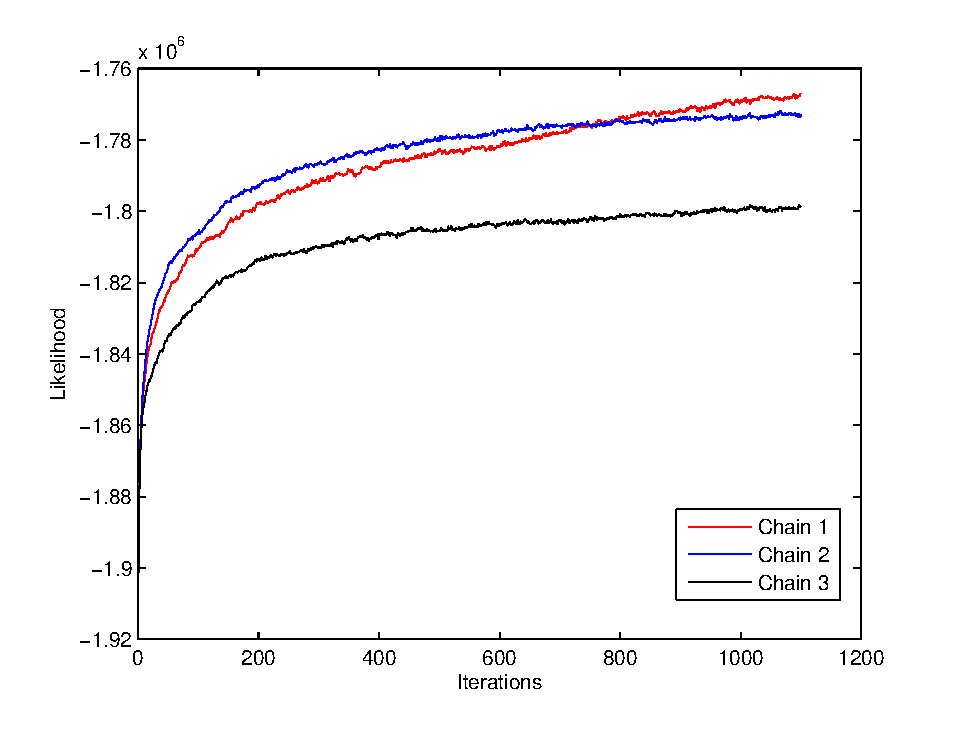
\includegraphics[scale=1.0]{lda_plot}
		\end{center}
	\end{figure}

	\begin{figure}
		\begin{center}
			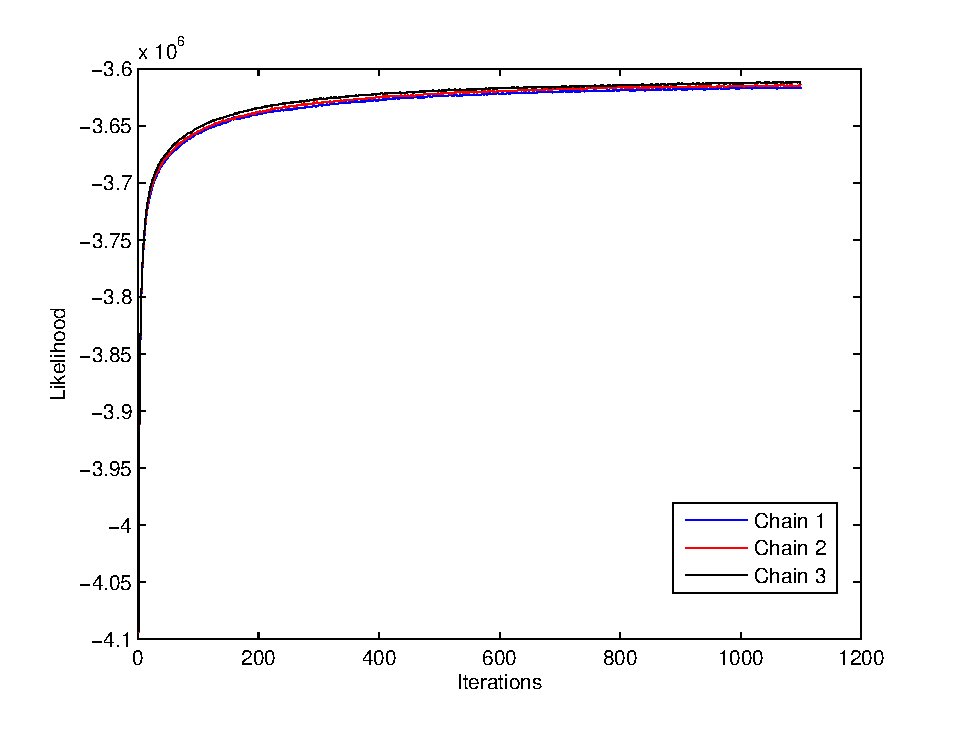
\includegraphics[scale=1.0]{bigram_plot}
		\end{center}
	\end{figure}
	
	
	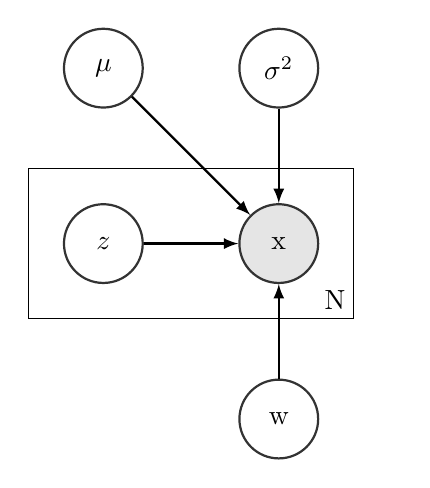
\begin{tikzpicture}
	\tikzstyle{main}=[circle, minimum size = 10mm, thick, draw =black!80, node distance = 12mm]
\tikzstyle{connect}=[-latex, thick]
\tikzstyle{box}=[rectangle, draw=black!100]
  \node[main, fill = white!100] (z) [] {$z$};
  \node[main, fill = black!10] (x) [right=of z] {x};
  \node[main] (mu) [above=of z] {$\mu$};
  \node[main] (sigma) [above=of x] {$\sigma^2$};
  \node[main] (w) [below=of x] {w};
  \path 
        (z) edge [connect] (x)
        (mu) edge [connect] (x)
        (sigma) edge [connect] (x)
        (w) edge [connect] (x);
  \node[rectangle, inner sep=0mm, fit= (z) (x),label=below right:N, xshift=10.5mm, yshift=0.5mm] {};
 \node[rectangle, inner sep=4.4mm,draw=black!100, fit= (z) (x)] {};

	\end{tikzpicture}


\end{document}